% =====================================================================
%  Chapter 3 -- Methodology
%  Structure follows the Experimental Section of Kwon (2025): setup,
%  design, modelling, then the experimental procedure.
% =====================================================================
\chapter{Methodology}
\label{ch:experimental}

The following sections detail the methodology used to evaluate
magnetohydrodynamically pumped Galinstan as a coolant for PECs. Two objectives
guided the work. The first is to compare the thermal performance of the
Galinstan cooling loop with that of a similar water cooling loop under
equivalent operating conditions (RQ1). The second is to quantify the influence
of a high-frequency magnetic leakage field on the Galinstan coolant (RQ2).
\Cref{sec:setup} describes the experimental setup, including the two cooling
loops, the instrumentation and the safety considerations.
\Cref{sec:inductor-design} presents the design of the power-dense inductor used
as the heat source in the second experiment. \Cref{sec:thermal-model} develops
the thermal models used to interpret the measurements, and
\cref{sec:programme} gives the procedures for the two experiments.

% ---------------------------------------------------------------------
\section{Experimental Setup}
\label{sec:setup}

\subsection{Cooling System Overview}
\label{sec:loop-overview}

Two cooling loops were used in this project, one circulating Galinstan and the
other water. Both follow the arrangement shown in \cref{fig:cooling-loop}. A
pump drives the coolant through a cold plate that interfaces with the heat
source, and then through a fan-cooled radiator, where the heat is rejected to
the environment. A flow sensor in the hot line measures the coolant flow rate.

\begin{figure}[htbp]
  \centering
  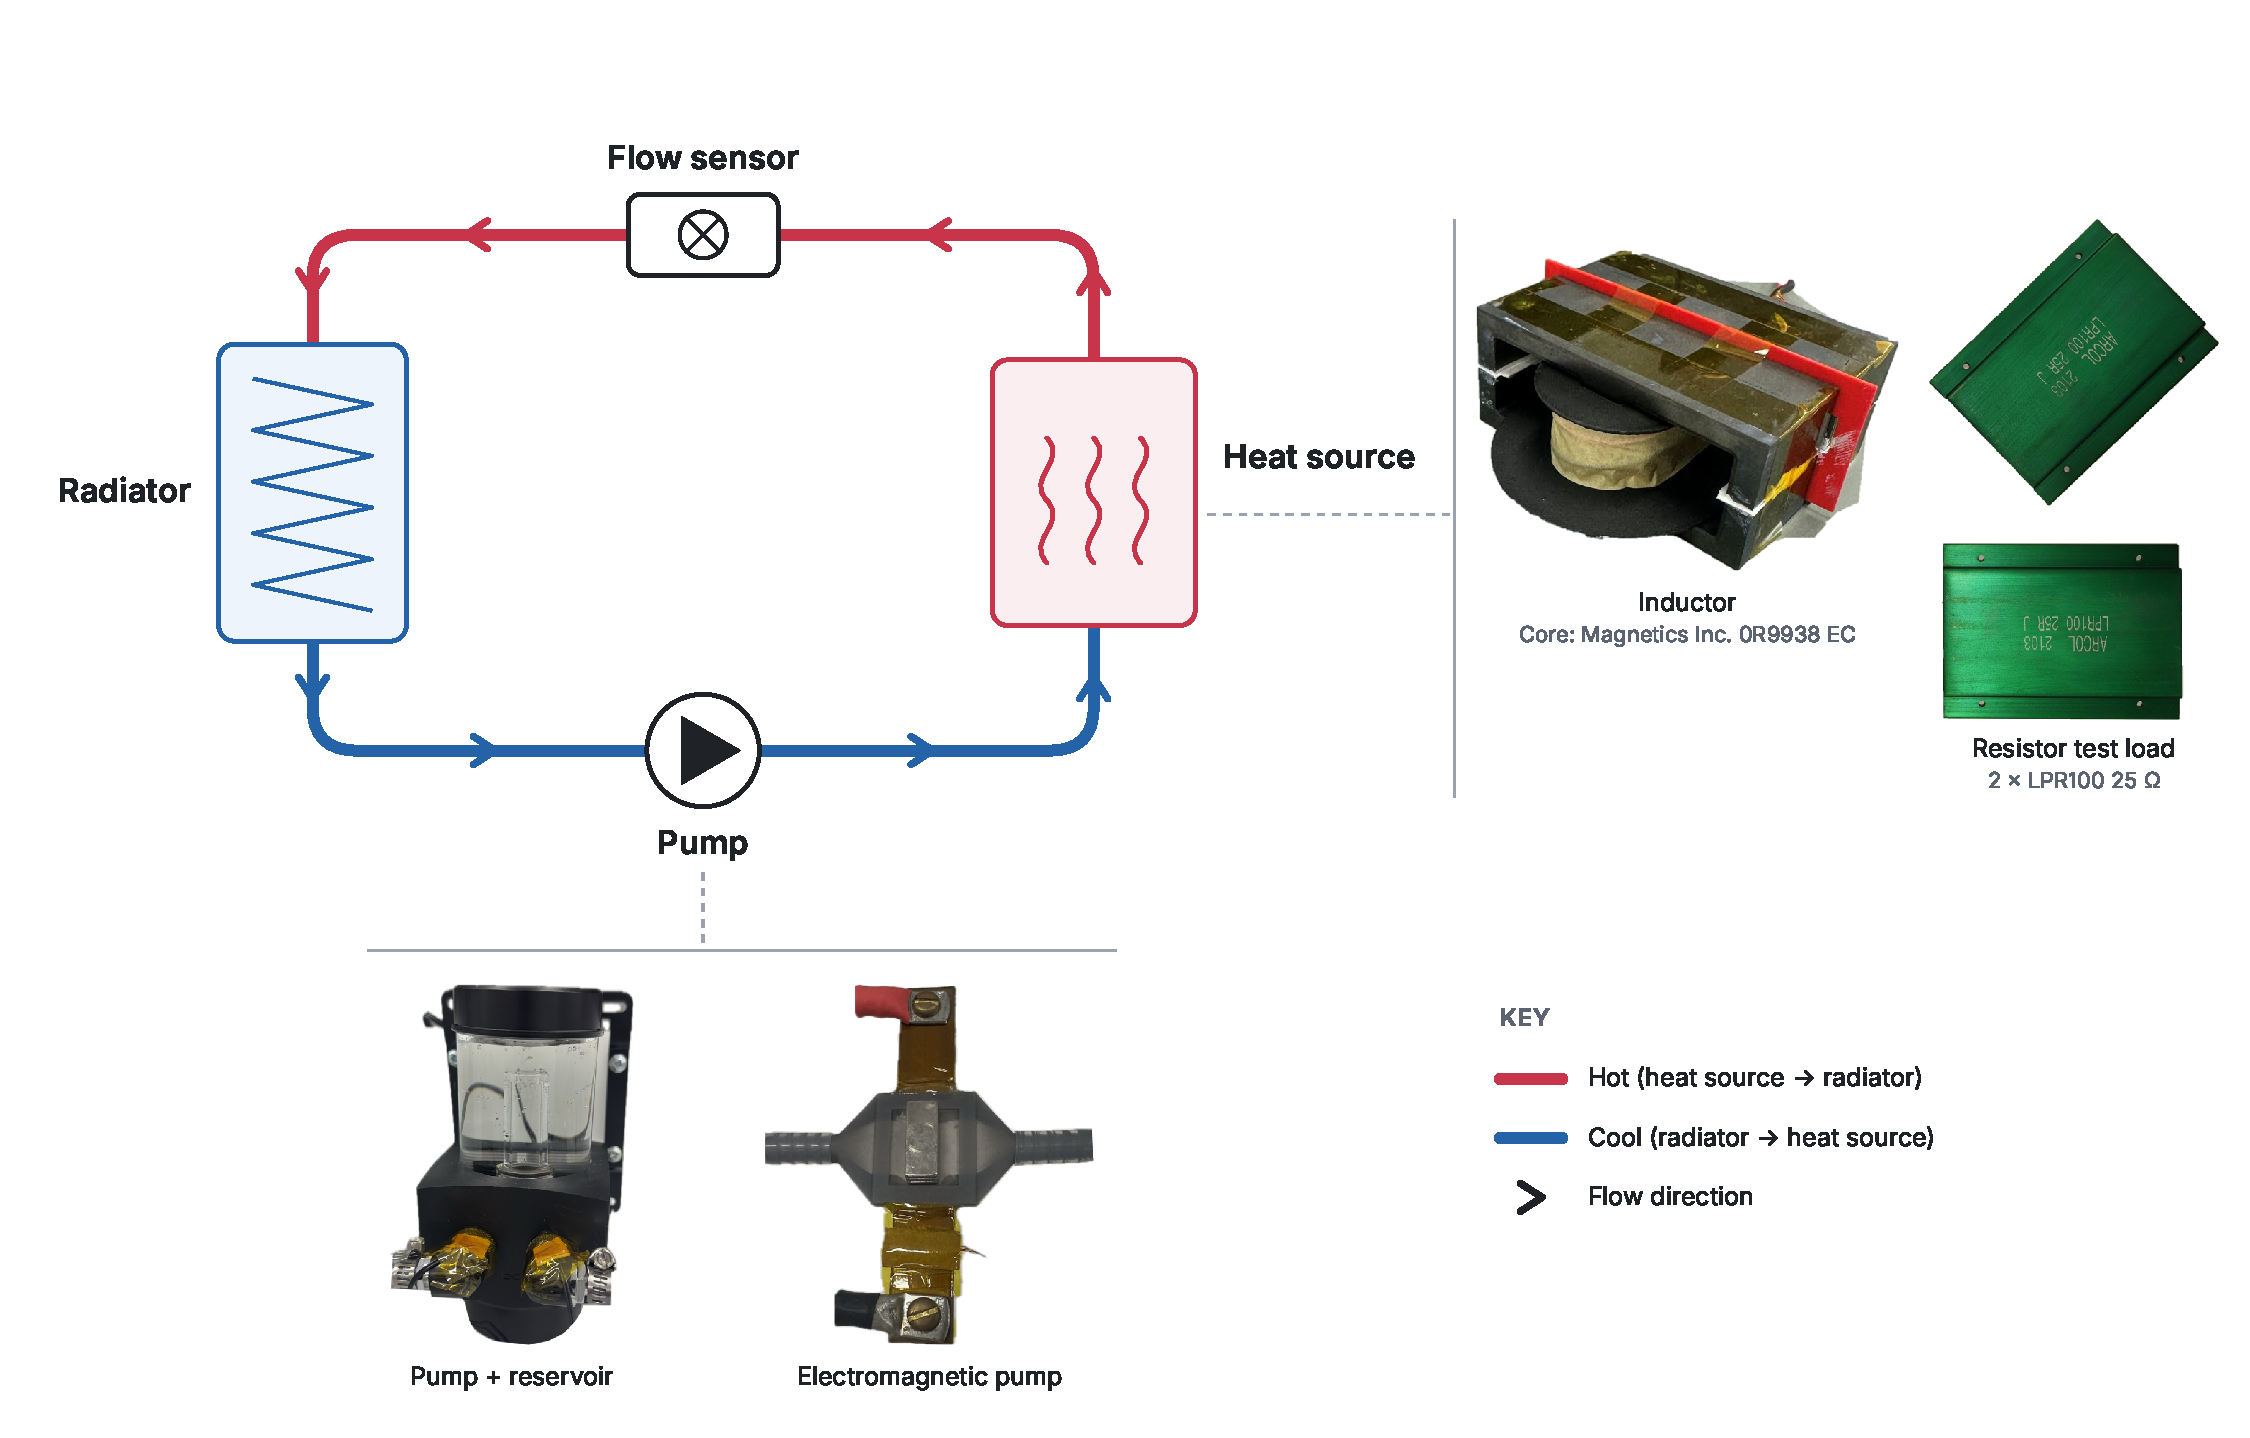
\includegraphics[width=0.85\linewidth]{figures/cooling_loop.pdf}
  \caption{Cooling loop arrangement shared by the Galinstan and water systems.
    The coolant is pumped through the heat source (resistor test load or
    inductor), past the flow sensor and through the radiator before returning
    to the pump. The water loop uses a pump with an integrated reservoir; the
    Galinstan loop uses an electromagnetic pump.}
  \label{fig:cooling-loop}
\end{figure}

The Galinstan loop is the apparatus constructed by the 2025 Part~IV Project~\#51
group~\cite{kwon_project_2025,loh_project_2025}. Galinstan is circulated by a
permanent-magnet DC conduction pump, in which a current passed through the
coolant between two copper electrodes produces a Lorentz force
(\cref{sec:em-pumping}). The pump is supplied by a XANTREX XKW~60--18 DC power
supply, which provides up to \SI{18}{\ampere}. PFA tubing carries the coolant
to an ATS-TCP-1001 tubed cold plate and back through an ATS-TCP-1003 cold plate
fitted with a heat sink and two fans, which acts as the
radiator~\cite{kwon_project_2025,advanced_thermal_solutions_inc_tubed_2021}.
Conventional mechanical flow meters are not compatible with Galinstan, so the
flow rate is measured with an electromagnetic flow sensor of the same
construction as the pump. The flowing coolant induces an EMF $E$ across the
sensor electrodes, from which the volumetric flow rate is $\Vdot = Eh/B$, where
$h$ is the channel height and $B$ the magnetic flux density across the
channel~\cite{kwon_project_2025}.

The water loop was designed and built by the project partner, Ekbote, to
replicate the Galinstan apparatus, and its design is detailed in Ekbote's
project report~\cite{ekbote_project_2026}. It uses the same model of tubed cold
plate (ATS-TCP-1001), so that the two
coolants are compared through an identical cold-plate geometry
(\cref{tab:coolant-properties}). The water is circulated by a pump with an
integrated reservoir, whose speed is set by the duty cycle of its drive signal,
and the flow rate is read directly from a Sea Zhongjiang digital flow meter. A
valve was later added to the water loop to reduce the flow below the
controllable range of the pump. The two loops therefore share the heat source
and the cold-plate geometry, but differ in the pump, the achievable flow range
and the method of flow measurement.

\subsection{Heat Sources}
\label{sec:heat-sources}

Two heat sources were used. For the first experiment, heat was applied by two
\SI{100}{\watt}, \SI{25}{\ohm} ARCOL LPR100 resistors mounted side by side on the
cold plate with a thermal interface material. The resistors were connected in
series and supplied by a GW Instek GPE-3323 DC power supply, so that the
dissipated power could be read directly from the supply. A heat load of
\SI{72}{\watt} (\SI{60}{\volt} across the \SI{50}{\ohm} pair) was used for most
tests, the same load used in~\cite{kwon_project_2025,loh_project_2025}. The
resistors were covered with polystyrene insulation to reduce the heat lost to
the environment. For the second experiment, the resistors were replaced by a
power-dense planar inductor, whose design is described in
\cref{sec:inductor-design}.

\subsection{Instrumentation}
\label{sec:instrumentation}

Galinstan is corrosive to many commonly used sensor materials, which restricts
the range of compatible measurement devices (\cref{sec:compatibility}). System
performance was therefore evaluated using the limited set of measurements
summarised in \cref{tab:measurements}. Temperatures around each loop were
logged continuously by a thermistor data-acquisition system adapted
from~\cite{kwon_project_2025,loh_project_2025}. At steady state, K-type
thermocouples, with an accuracy of $\pm\SI{2.2}{\celsius}$~\cite{loh_project_2025},
were used as the reference temperatures at the resistor, the cold-plate inlet
and the cold-plate outlet. A thermal camera was used where available, chiefly
for the inductor experiment.

\begin{table}[htbp]
  \centering
  \caption{Measured quantities and instrumentation.}
  \label{tab:measurements}
  \small
  \begin{tabularx}{\linewidth}{@{}>{\raggedright\arraybackslash}p{2.7cm}
      >{\raggedright\arraybackslash}p{4.1cm} L@{}}
    \toprule
    Quantity & Description & Method \\
    \midrule
    \multirow[t]{2}{=}{Heat load}
      & Power dissipated by the resistors.
      & Read from the GW Instek GPE-3323 DC power supply. \\
      & Power dissipated in the inductor.
      & Estimated from the core-loss model and the measured AC resistance
        (\cref{sec:model-validation}). \\
    \midrule
    \multirow[t]{2}{=}{Volumetric flow rate, $\Vdot$}
      & Galinstan loop.
      & EMF $E$ of the electromagnetic flow sensor, read with an Agilent 34410A
        digital multimeter; $\Vdot = Eh/B$~\cite{kwon_project_2025}. \\
      & Water loop.
      & Read directly from the Sea Zhongjiang digital flow meter. \\
    \midrule
    Temperature
      & Thermistors around the loop and, at steady state, thermocouples at the
        resistor, cold-plate inlet and cold-plate outlet.
      & Data-acquisition system adapted from~\cite{kwon_project_2025,loh_project_2025};
        thermal camera where available. \\
    \midrule
    Pump power
      & Electrical input power to each pump.
      & Voltage across the pump terminals and current from each pump's DC
        power supply. \\
    \midrule
    AC resistance, $R_{\mathrm{ac}}$
      & Series resistance of the inductor winding.
      & Agilent E4980A LCR meter (\cref{sec:exp2}). \\
    \midrule
    Pump volume
      & Volume occupied by each pump.
      & Physical measurement, supplemented by CAD dimensions where physical
        measurement is impractical. \\
    \bottomrule
  \end{tabularx}
\end{table}

\subsection{Safety Considerations}
\label{sec:safety}

The safety of project members and other laboratory users was prioritised
throughout the experimental setup and operation. Every experiment was set up by
two project members, and all connections were cross-checked with the project
partner before the system was energised. While temperatures exceeded
\SI{38}{\celsius}, the apparatus was continuously monitored by at least one
project member, and no one was permitted to interact with the system while it
was live. All electrical terminals operating above \SI{50}{\volt} DC were
covered, and the inverter and resonant tank used in the second experiment were
fully enclosed in acrylic boxes. Protective eyewear was worn, and physical
barriers prevented accidental contact with the live system. At shutdown, the
heat source was switched off first while the coolant continued to circulate,
and the apparatus was supervised for at least 30 minutes, until it had cooled
below \SI{38}{\celsius}.

% ---------------------------------------------------------------------
\section{Inductor Design}
\label{sec:inductor-design}

Cooling systems for magnetic components sit in their leakage fields
(\cref{sec:form-factor}), which could heat a Galinstan coolant. An initial ANSYS
simulation, with the Galinstan modelled as a stationary solid, found it 3.2
times as lossy as aluminium and almost 3.9 times as lossy as copper, and showed
that \SI{1}{\milli\metre} of copper shielding reduced the total loss by over
\SI{70}{\percent}. To measure this effect, a power-dense inductor that requires
active cooling was built and placed on the Galinstan cold plate. It operates at
\SI{85}{\kilo\hertz}~\cite{society_of_automotive_engineers_r_2024}, so that its
leakage field is representative of IPT magnetics (\cref{sec:ipt-losses}), and
uses a planar geometry, which offers better thermal performance than
alternatives such as pot cores. The final construction is shown in
\cref{fig:inductor-photo}.

\subsection{Analytical and Numerical Design}
\label{sec:analytical-design}

To reduce computation time and narrow the design space, an analytical model was
developed before the numerical simulations. This initial model assumed a
two-part construction of TDK N85 ferrite ELP-type cores, and swept the air-gap
length (\SIrange{0.5}{1.5}{\milli\metre}) and the number of turns (8--12). The
core loss of each design was estimated with the Steinmetz equation, which
expresses the loss per unit volume as a power law in frequency and peak flux
density~\cite{li_review_2022}. The model identified designs whose loss exceeds
the core's datasheet loss limit of
\SI{17.88}{\watt}~\cite{magnetics_inc_specification_2005}, so that active
cooling is required, while keeping the peak flux density below about
\SI{300}{\milli\tesla}.

An ANSYS model was then constructed and run as a two-parameter sweep over
air-gap length and number of turns. It was later found that the available cores
were Magnetics Inc.\ Material~R rather than the assumed TDK N85. A custom
material definition was therefore created by modifying the properties of TDK
N95, which are similar to those of Material~R. The core material was assumed to
operate at \SI{65}{\celsius}, the target steady-state operating temperature for
the experiments. With the material defined, a parameter sweep (8--12 turns,
\SIrange{0.5}{1.2}{\milli\metre} air gap) was performed to extract the
inductance and core loss.

To finalise the design, the flux density in the core was checked and found to
be acceptable, within the linear region of operation (\cref{fig:flux-density}).
The final design parameters, including the inductance and core loss of the
chosen design, are given in \cref{tab:inductor-design}.

\begin{figure}[htbp]
  \centering
  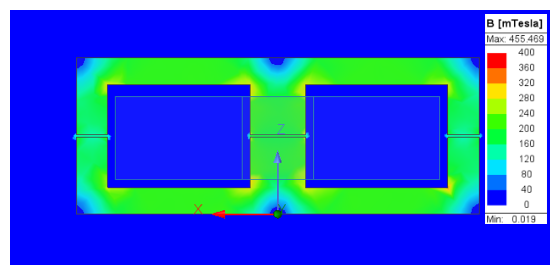
\includegraphics[width=0.72\linewidth]{inductor_flux_density}
  \caption{Magnetic flux density in the selected inductor design ($N = 8$,
    $l_{\mathrm{g}} = \SI{0.6}{\milli\metre}$).}
  \label{fig:flux-density}
\end{figure}

\begin{table}[htbp]
  \centering
  \caption{Final inductor parameters from the ANSYS model at the rated current
    of \SI{12}{\ampere} rms.}
  \label{tab:inductor-design}
  \begin{tabular}{@{}lll@{}}
    \toprule
    Parameter & Value & Unit \\
    \midrule
    Core geometry  & Magnetics Inc.\ 0\,9938\,EC & -- \\
    Core material  & Magnetics Inc.\ Material~R  & -- \\
    Air-gap length & 0.6   & \si{\milli\metre} \\
    Turns          & 8     & -- \\
    Inductance     & 92.5  & \si{\micro\henry} \\
    Core loss      & 30.81 & \si{\watt} \\
    \bottomrule
  \end{tabular}
\end{table}

\subsection{Model Validation}
\label{sec:model-validation}

Once the inductor had been built (\cref{fig:inductor-photo}), measurements were
taken to design the LCC tuning required to drive the desired resonant current.
These measurements also serve to validate the model, whose values at the rated
current of \SI{12}{\ampere} rms are given in \cref{tab:inductor-design}.

\begin{figure}[htbp]
  \centering
  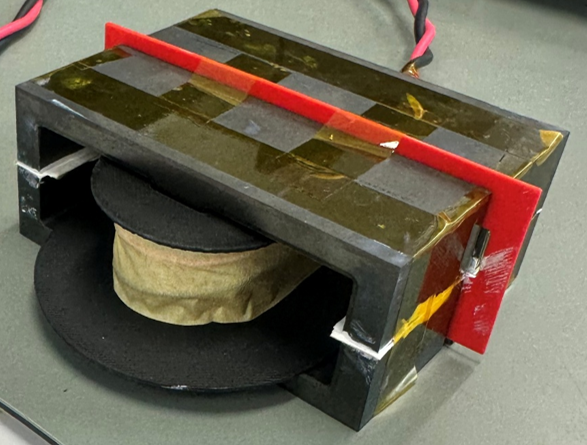
\includegraphics[width=0.42\linewidth]{inductor_photo}
  \caption{Constructed planar inductor.}
  \label{fig:inductor-photo}
\end{figure}

The inductance was measured as \SI{92.1}{\micro\henry}, within \SI{1}{\percent}
of the simulation model, although this measurement included the effect of long
leads, which would be expected to increase it. The AC resistance
$R_{\mathrm{ac}}$, which determines the winding loss, was measured with an LCR
meter at low excitation as \SI{83}{\milli\ohm}, giving a winding loss of
\SI{11.95}{\watt} at \SI{12}{\ampere} rms.

For a heat transfer investigation in which temperatures are continuously
monitored, some uncertainty in the loss estimate is acceptable. For the later
experiments, the total inductor loss is therefore taken as \SI{42.76}{\watt}
(\SI{30.81}{\watt} core loss plus \SI{11.95}{\watt} winding loss).

\subsection{Thermal Considerations and Cooling Strategy}
\label{sec:inductor-thermal}

The main constraint was asymmetric cooling. The upper core relies on convection
to ambient air, while the lower core sits on the cold plate, and the air gap
between them acts as a thermal insulator. Thermal paste was applied between the
upper and lower cores to reduce the temperature difference and improve heat
transfer to the cooling system. Although not optimal, this configuration is
suitable for the second experiment, which aims to demonstrate Galinstan cooling
of a power-dense inductor and to assess the leakage-field interaction rather
than to produce the best-performing system. Future work could improve the design
by cooling both the top and bottom cores, or by using asymmetric core designs
with an integrated heat-transfer path, such as the inductor of Gao
\emph{et al.}~\cite{gao_modeling_2022}.

\subsection{Capacitor Tuning}
\label{sec:capacitor-tuning}

The allowable reactance of the inductor was limited by the maximum voltage
developed across the series tuning capacitors needed to boost the volt-amperes
(VA) in the inductor, which was limited to \SI{150}{\volt} across any single
capacitor. To find
acceptable tuning values, an optimisation model was developed using the Solver
add-in in Microsoft Excel, which made it possible to check quickly whether a
given inductance was feasible or would cause the capacitor voltage to exceed its
rating.

The target capacitance is given by
\begin{equation}
  C_{\mathrm{target}} = \frac{1}{2\pi f \left(2\pi f L_{1} - X_{\mathrm{res}}\right)},
  \label{eq:c-target}
\end{equation}
where $f$ is the resonant frequency of the network (\SI{85}{\kilo\hertz}),
$L_{1}$ is the inductance of the primary magnetics and $X_{\mathrm{res}}$ is the
resonant reactance of the system. $X_{\mathrm{res}}$ sets the resonant current in
the primary magnetics, as given by
\begin{equation}
  X_{\mathrm{res}} = \frac{2\sqrt{2}\, V_{\mathrm{DC}}}{\pi I_{1}},
  \label{eq:x-res}
\end{equation}
where $I_{1}$ is the desired resonant current and $V_{\mathrm{DC}}$ is the DC bus
voltage, here \SI{60}{\volt}. \Cref{eq:x-res} is valid only for a conduction
angle of \SI{180}{\degree}. With the measured inductance of \SI{92.1}{\micro\henry} and a resonant current of
\SI{12}{\ampere}, \cref{eq:c-target,eq:x-res} give a target capacitance of
\SI{41.90}{\nano\farad}.

Initially, the optimisation model selected a single capacitor value for the
entire board. The result was relatively poor, with the best design differing by
\SI{8.11}{\percent} from the target capacitance. The model was then extended to
allow one value from a limited set (\SIlist{22;68;100}{\nano\farad}) to be
selected for each of the four series-connected rows of the tuning board, with up
to 14 capacitors in parallel per row. This reduced the detuning to
\SI{2.12}{\percent} of the target value. The final arrangement, with the voltage
across each row at the rated current, is given in \cref{tab:capacitor-opt}. The
highest row voltage is about \SI{146}{\volt}, within the \SI{150}{\volt} limit.

\begin{table}[htbp]
  \centering
  \caption{Final arrangement of the series tuning capacitors from the
    optimisation model. The four rows are connected in series; row voltages are
    at \SI{12}{\ampere} rms and \SI{85}{\kilo\hertz}.}
  \label{tab:capacitor-opt}
  \small
  \begin{tabular}{@{}lcccc@{}}
    \toprule
    Row & Capacitor value & Number in parallel & Row capacitance & Row voltage \\
        & (\si{\nano\farad}) & & (\si{\nano\farad}) & (\si{\volt}) \\
    \midrule
    1 & 22 & 7 & 154 & 145.9 \\
    2 & 68 & 3 & 204 & 110.1 \\
    3 & 22 & 7 & 154 & 145.9 \\
    4 & 22 & 7 & 154 & 145.9 \\
    \midrule
    \multicolumn{3}{@{}l}{Target capacitance}   & 41.90 & \\
    \multicolumn{3}{@{}l}{Achieved capacitance} & 41.01 & \\
    \multicolumn{3}{@{}l}{Error}                & 0.89 (\SI{2.12}{\percent}) & \\
    \bottomrule
  \end{tabular}
\end{table}

% ---------------------------------------------------------------------
\section{Thermal Modelling}
\label{sec:thermal-model}

Thermal models were developed alongside the experiments, both to interpret the
measurements and to extend them beyond the conditions the apparatus could reach.
This section first presents a lumped thermal network and the $\varepsilon$--NTU
analysis used to calculate its cold-plate resistance, followed by the convection
correlations and test conditions it relies on. A conjugate heat transfer
simulation, which resolves the temperature field that the network lumps
together, is then described. The models are compared with the measurements in
\cref{ch:results}.

\subsection{Thermal Network}
\label{sec:thermal-network}

Following the analyses of Kwon~\cite{kwon_project_2025} and
Loh~\cite{loh_project_2025}, the input heat $\Qin$ divides at the resistor node
$\Tres$, as shown in \cref{fig:thermal-network}. Part of the heat is
lost to ambient through $\Rmisc$. The rest, $\Qplate$, passes through the
package resistance $\Rpack$ (resistor and thermal interface) to a fictitious
isothermal plate node $T_{\mathrm{P}}$, and then through the cold-plate
resistance $\Rcp$ to the coolant inlet:
\begin{equation}
  \Qin = \frac{\Tres - T_{\mathrm{A}}}{\Rmisc}
       + \frac{\Tres - \Tin}{\Rpack + \Rcp}.
  \label{eq:network}
\end{equation}
The resistance to ambient $\Rmisc$ was found for each loop from a no-flow test
at a heat load of \SI{12}{\watt}. With no coolant flow, the heat input is lost
to the environment, so
\begin{equation}
  \Rmisc = \frac{\Tres - T_{\mathrm{A}}}{\Qin}.
  \label{eq:rmisc}
\end{equation}
This resistance was then used to calculate the loss to the environment at any
resistor temperature. For the Galinstan loop, $T_{\mathrm{A}} =
\SI{20.5}{\celsius}$ and $\Rmisc = \SI{3.33}{\celsius\per\watt}$; for the water
loop, $T_{\mathrm{A}} = \SI{21.6}{\celsius}$ and
$\Rmisc = \SI{2.95}{\celsius\per\watt}$. With these values, between
\SI{9}{\watt} and \SI{12}{\watt} of the heat load is lost to the environment in
each test (\cref{tab:measured-performance}). This network was used in all the
following models.
\issue{\Cref{fig:thermal-network} still labels the resistor node
$T_{\mathrm{M}}$; update the image to $T_{\mathrm{resistor}}$.}

\begin{figure}[htbp]
  \centering
  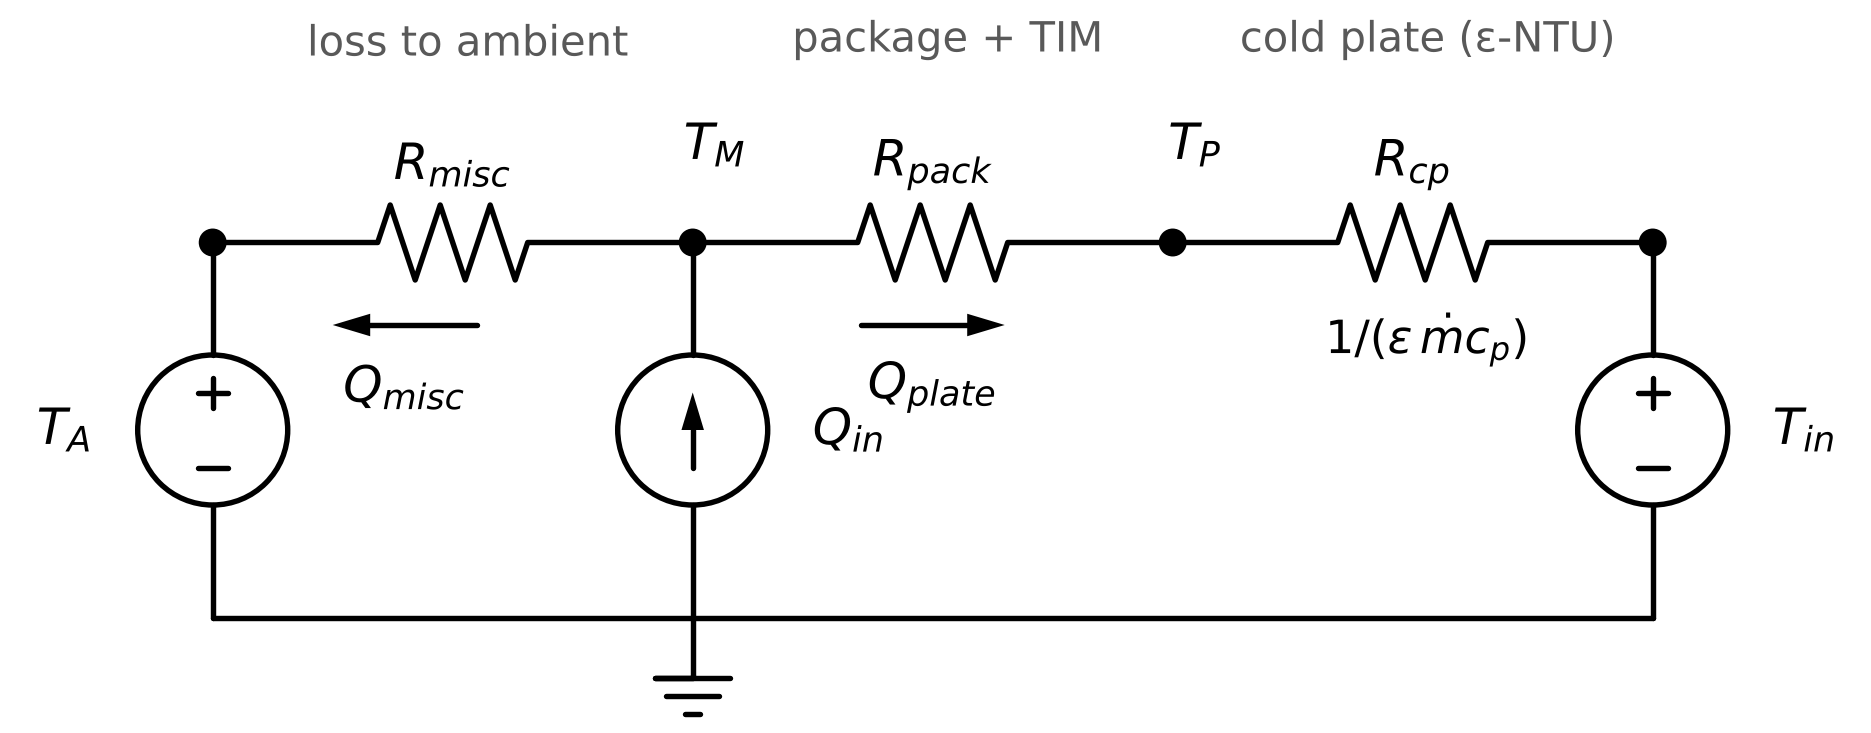
\includegraphics[width=0.85\linewidth]{thermal_network}
  \caption{Thermal network as an electrical analogue (temperature $\equiv$
    potential, heat flow $\equiv$ current); $T_{\mathrm{A}}$ and $\Tin$ are fixed
    boundary conditions.}
  \label{fig:thermal-network}
\end{figure}

\subsection{\texorpdfstring{$\varepsilon$--NTU}{epsilon-NTU} Analysis of the Cold Plate}
\label{sec:eps-ntu}

For this analysis, the plate is considered isothermal at $T_{\mathrm{P}}$, so
coolant entering at $\Tin$ approaches the plate temperature exponentially. An
energy balance on a tube element of perimeter $P$ gives~\cite{bergman_fundamentals_2017}
\begin{equation}
  \frac{T_{\mathrm{P}} - T_{\mathrm{f}}(x)}{T_{\mathrm{P}} - \Tin}
    = \exp\!\left(-\frac{hPx}{\mdot\,\cp}\right).
  \label{eq:temp-profile}
\end{equation}
At the outlet ($x = L$, $PL = A$), the exponent is defined as the number of
transfer units, $\NTU = hA/(\mdot\,\cp)$. This is the ratio of the
wall-to-coolant convective conductance to the heat-capacity rate of the coolant.
Each transfer unit reduces the remaining plate-to-coolant temperature difference
by a factor of $e$, so the coolant absorbs about \SI{63}{\percent} of the maximum
possible heat after one transfer unit~\cite{bergman_fundamentals_2017}. Defining
the effectiveness $\varepsilon$ as this fraction gives
\begin{equation}
  \Qplate = \varepsilon\,\mdot\,\cp\,(T_{\mathrm{P}} - \Tin), \qquad
  \varepsilon = 1 - e^{-\NTU}, \qquad
  \Rcp = \frac{1}{\varepsilon\,\mdot\,\cp},
  \label{eq:effectiveness}
\end{equation}
\begin{equation}
  T_{\mathrm{P}} = \Tin + \Qplate\Rcp, \qquad
  \Tout = \Tin + \frac{\Qplate}{\mdot\,\cp}.
  \label{eq:plate-outlet}
\end{equation}
This is the effectiveness relation for one flow stream against an isothermal
surface~\cite{bergman_fundamentals_2017}. Its limits show whether a coolant is
limited by convection at the wall or by its ability to transport heat
(caloric-limited), as summarised in \cref{tab:ntu-regimes}.

\begin{table}[htbp]
  \centering
  \caption{Limiting regimes of the $\varepsilon$--NTU relation for an isothermal
    plate.}
  \label{tab:ntu-regimes}
  \small
  \begin{tabular}{@{}lllll@{}}
    \toprule
    Regime & NTU & $\varepsilon$ & $\Rcp$ & Lever to reduce $\Rcp$ \\
    \midrule
    Convection-limited & $\ll 1$ & $\approx \NTU$ &
      $\approx 1/(hA) + 1/(2\mdot\,\cp)$ & Raise $hA$ (Nu, area) \\
    Transitional & $\approx 1$ & $1 - e^{-\NTU}$ &
      $1/(\varepsilon\,\mdot\,\cp)$ & Both \\
    Caloric-limited & $\gg 1$ ($\gtrsim 3$) & $\to 1$ &
      $\to 1/(\mdot\,\cp)$ & Raise $\mdot\,\cp$ (flow rate) \\
    \bottomrule
  \end{tabular}
\end{table}

The isothermal-plate assumption relies on in-plane heat spreading within the
\SI{15}{\milli\metre} 6063 aluminium base (\cref{fig:coldplate-heatflow}). The
assumption weakens as the coolant temperature rise between inlet and outlet,
$\Delta T_{\mathrm{cool}} = \Qplate/(\mdot\,\cp)$, increases. The predicted rise
is below \SI{2}{\celsius} for water but approximately
\SIrange{17}{20}{\celsius} for Galinstan, so the model is expected to describe
water better than Galinstan. For this reason, the package resistance $\Rpack$
was calibrated on the two turbulent water tests, which give the most nearly
isothermal plate, as \SI{0.242}{\celsius\per\watt}. It was then held at this
value for all flows and both coolants.

\begin{figure}[htbp]
  \centering
  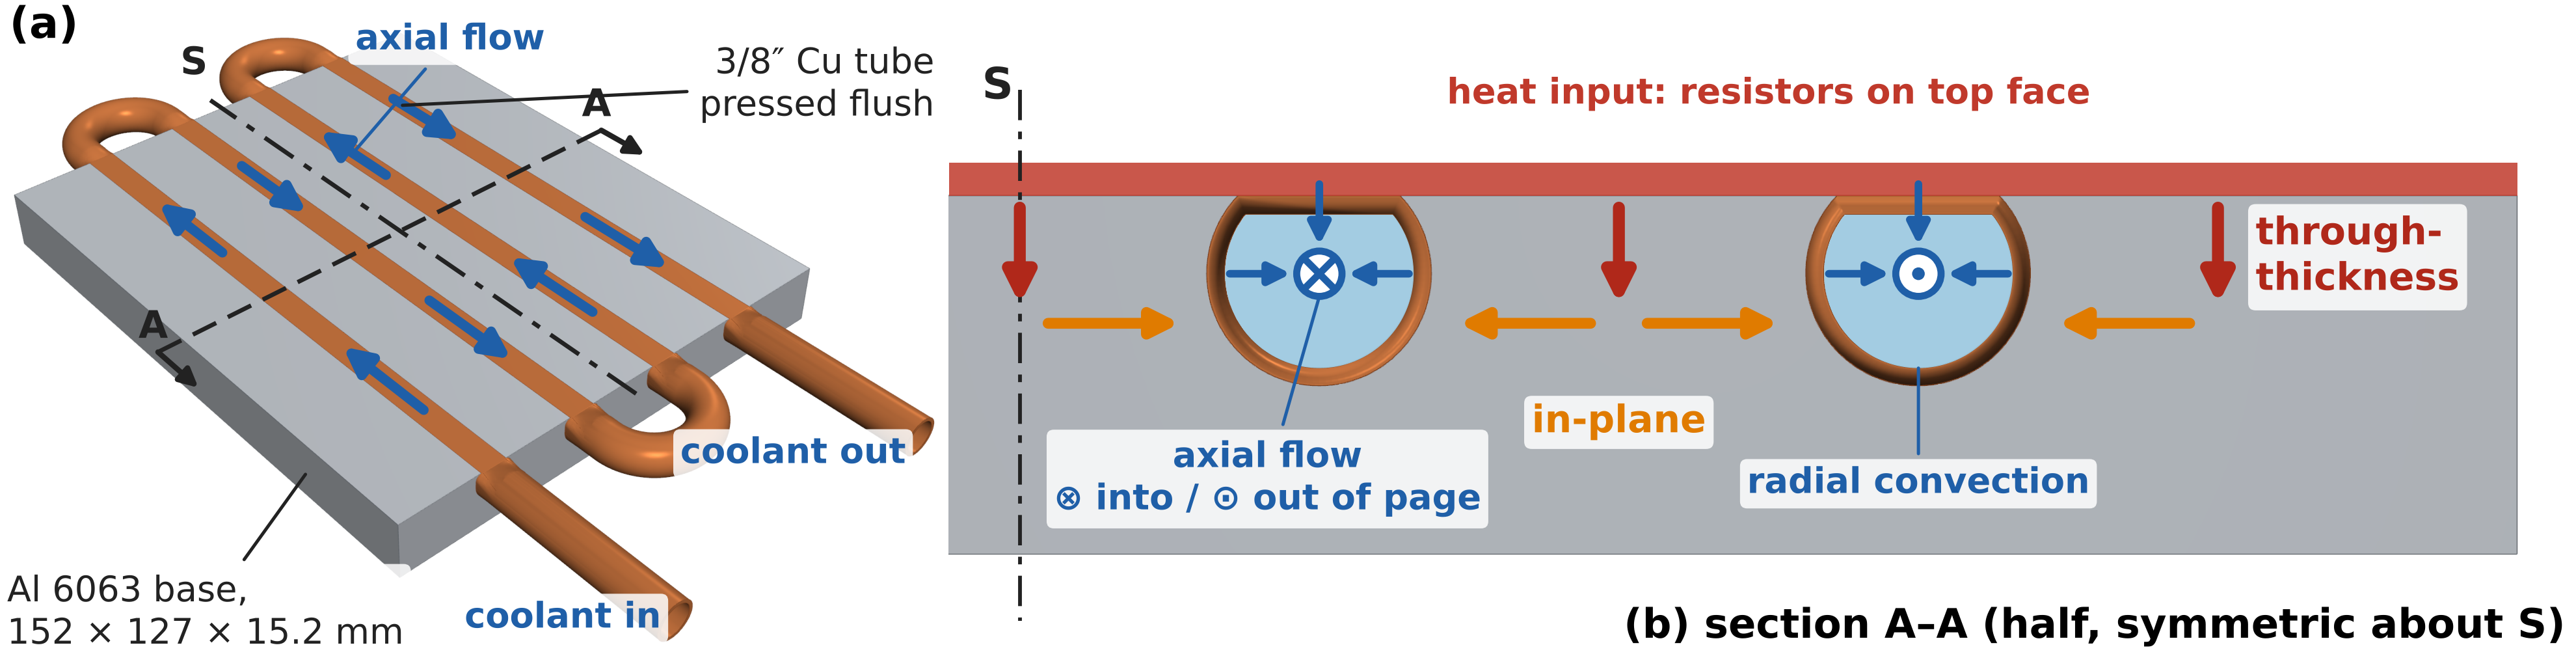
\includegraphics[width=0.85\linewidth]{coldplate_heat_flow}
  \caption{Heat-flow directions in the cold plate: in-plane spreading (plate),
    through-thickness conduction (part of $\Rpack$), axial flow and radial
    convection ($R_{\mathrm{conv}}$).}
  \label{fig:coldplate-heatflow}
\end{figure}

\subsection{Convection Correlations and Test Conditions}
\label{sec:convection}

The $\varepsilon$--NTU model requires an estimate of the heat transfer
coefficient $h$ between the tube wall and the coolant. It is obtained from
standard correlations for the Nusselt number, $\mathrm{Nu} = hD/k$, a
dimensionless measure of how effectively the flowing coolant removes heat from
the wall. For laminar flow, the Shah and London
correlation~\cite{shah_laminar_1978} gives the mean Nu along a tube at constant
wall temperature, including the thermal entry region where heat transfer is
highest. It is applied to each \SI{152}{\milli\metre} pass separately, on the
assumption that the U-bends mix the flow. For turbulent water
($\mathrm{Re} \geq 4000$), Gnielinski's correlation~\cite{bergman_fundamentals_2017}
is used, and no estimate is made in the transitional range
$2300 < \mathrm{Re} < 4000$. Galinstan remains laminar up to
\SI{5}{\milli\litre\per\second} ($\mathrm{Re} \leq 2110$). The correlations and
worked calculations for both coolants are given in \cref{app:convection}.

The NTU analysis uses these correlations for both coolants. For the turbulent
water tests, however, the cold-plate resistance given in the ATS-TCP-1001
datasheet~\cite{advanced_thermal_solutions_inc_tubed_2021} was later found to
fit the measured data better, so the temperature predictions for these tests
use the datasheet values, fitted as
$\Rcp = 0.0274\,\Vdot^{-0.415}$~\si{\kelvin\per\watt} ($\Vdot$ in
\si{\litre\per\minute}). The Galinstan and laminar water tests use the
$\varepsilon$--NTU model.
\Cref{tab:coolant-properties,tab:tests} summarise the cold-plate geometry, the
coolant properties and the test conditions.

\begin{table}[htbp]
  \centering
  \caption{Cold-plate geometry (ATS-TCP-1001) and coolant properties.}
  \label{tab:coolant-properties}
  \small
  \begin{tabularx}{\linewidth}{@{}>{\raggedright\arraybackslash}p{4.3cm}ll L@{}}
    \toprule
    Quantity & Galinstan & Water & Note \\
    \midrule
    Tube bore / heated length per pass & \SI{8}{\milli\metre} / \SI{152}{\milli\metre}
      & \SI{8}{\milli\metre} / \SI{152}{\milli\metre}
      & Bore measured; plate length and 4 passes
        from~\cite{advanced_thermal_solutions_inc_tubed_2021};
        $A = \SI{0.0153}{\metre\squared}$ \\
    $\rho$ (\si{\kilogram\per\metre\cubed}) / $\cp$ (\si{\joule\per\kilogram\per\kelvin})
      & 6370 / 366 & 1000 / 4182
      & Galinstan $\rho$~\cite{kwon_project_2025}, $\cp$~\cite{zhang_experimental_2019} \\
    $k$ (\si{\watt\per\metre\per\kelvin}) / $\mu$ (\si{\milli\pascal\second})
      & 16.5 / 2.4 & 0.60 / 1.0 & \cite{kwon_project_2025} \\
    \bottomrule
  \end{tabularx}
\end{table}

\begin{table}[htbp]
  \centering
  \caption{Steady-state tests, estimated coolant temperature rise and cold-plate
    resistance used in the predictions.}
  \label{tab:tests}
  \small
  \setlength{\tabcolsep}{4.5pt}
  \begin{tabular}{@{}llrrlrr@{}}
    \toprule
    Test & Flow & $\Qin$ (\si{\watt}) & Re & Regime &
      $\Delta T_\mathrm{cool}$ (\si{\celsius}) & $R_\mathrm{cp}$ (\si{\celsius\per\watt}) \\
    \midrule
    Galinstan, full (\SI{18}{\ampere}) & \SI{1.4}{\milli\litre\per\second}  & 72 & 591  & Laminar   & 17.8\textsuperscript{\textdagger} & 0.295 \\
    Galinstan, low (\SI{9}{\ampere})   & \SI{0.75}{\milli\litre\per\second} & 40 & 317  & Laminar   & 17.1\textsuperscript{\textdagger} & 0.555 \\
    Water & \SI{3.5}{\litre\per\minute}  & 72 & 9284 & Turbulent & 0.26 & 0.016\textsuperscript{\textdaggerdbl} \\
    Water & \SI{1.75}{\litre\per\minute} & 72 & 4642 & Turbulent & 0.52 & 0.022\textsuperscript{\textdaggerdbl} \\
    Water & \SI{0.73}{\litre\per\minute} & 72 & 1936 & Laminar   & 1.22 & 0.074 \\
    Water & \SI{0.5}{\litre\per\minute}  & 72 & 1326 & Laminar   & 1.78 & 0.088 \\
    \bottomrule
    \multicolumn{7}{@{}p{\linewidth}@{}}{\footnotesize
      $\Delta T_\mathrm{cool} = Q_\mathrm{plate}/(\mdot\,\cp)$, where
      $Q_\mathrm{plate}$ is $\Qin$ less the loss to ambient through
      $R_\mathrm{misc}$. $R_\mathrm{cp}$ is from the $\varepsilon$--NTU model
      unless marked.
      \textsuperscript{\textdagger}\,Galinstan $\mdot\,\cp$ estimated from the
      energy balance, so $\Delta T_\mathrm{cool}$ equals the measured
      $T_\mathrm{out} - T_\mathrm{in}$; nominal flows are from the EMF
      flow sensor.
      \textsuperscript{\textdaggerdbl}\,ATS datasheet
      fit~\cite{advanced_thermal_solutions_inc_tubed_2021};
      \SI{1.75}{\litre\per\minute} is slightly extrapolated below the lowest
      datasheet point (\SI{1.89}{\litre\per\minute}).}
  \end{tabular}
\end{table}
\edited{Turbulent water flows changed from 3.6 and \SI{1.8}{\litre\per\minute}
to the measured 3.5 and \SI{1.75}{\litre\per\minute} (58.3 and
\SI{29.2}{\milli\litre\per\second}) here and in later chapters. Re and
$\Delta T_{\mathrm{cool}}$ were recalculated; $\Rcp$, NTU, $\Rpack$ and the
predicted temperatures are unchanged at the precision shown (the datasheet
$\Rcp$ changes by \SI{0.0002}{\celsius\per\watt}). Thermal\_Network\_Model.xlsx
still uses 3.6 and \SI{1.8}{\litre\per\minute}.}

\subsection{Conjugate Heat Transfer Simulation}
\label{sec:cht}

The thermal network reproduces the measured resistor temperatures by lumping the
cold plate into a single isothermal node. This is reasonable for water, but for
Galinstan the plate is not isothermal. The network also cannot resolve how heat
spreads from the discrete resistor footprints through the press-fit tube
contact, nor capture flow redevelopment at the U-bends or the transitional flow
suspected in the low-flow water tests. A conjugate heat transfer (CHT)
simulation, which solves the coolant flow and the conduction through the solids
together, was therefore completed in SimScale~\cite{simscale_gmbh_simscale_2021}.
It resolves the temperature fields in the plate and coolant, and the local peak
temperatures that govern component and insulation limits.

To reduce computation time, a simplified model of the cold plate was first
created in Onshape~\cite{ptc_onshape_2015} and imported into SimScale
(\cref{fig:cfd_setup}). An internal flow volume was then defined in the
geometry. The solids were assigned SimScale's default material properties for
aluminium and copper, and water used the default material. A custom Galinstan
material was created from the properties in \cref{tab:coolant-properties}. The
simulation settings and boundary conditions are summarised in
\cref{tab:simulation-setup}, and parameters not listed were left at their
default values.

\begin{figure}[htbp]
    \centering
    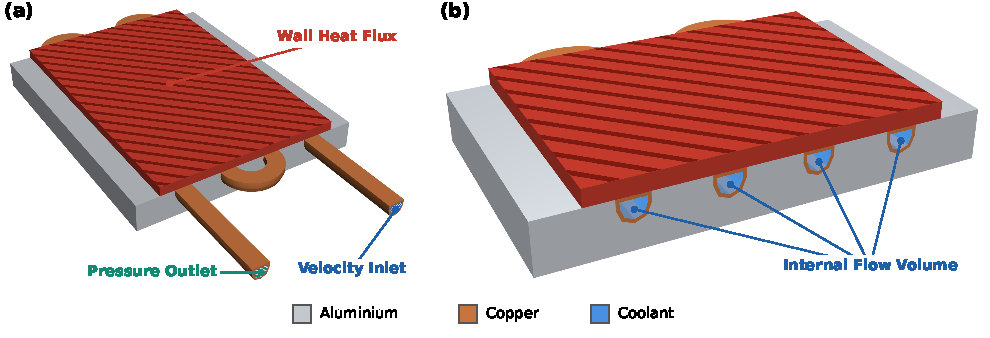
\includegraphics[width=\textwidth]{coldplate_figure.pdf}
    \caption{Cold-plate model used for the CHT analysis.
        (a)~Isometric view and (b)~cut showing the internal flow volume.}
    \label{fig:cfd_setup}
\end{figure}

The boundary conditions were chosen to match each test. The inlet was set as a
velocity inlet at the measured inlet temperature of the test (for example,
\SI{29.8}{\celsius} for the full-flow Galinstan test), with the velocity
adjusted to give the measured flow rate. The outlet was held at a pressure of
\SI{1}{atm}. The heat input was applied as a heat flux equal to the heat
reaching the cold plate, $\Qplate$, rather than the full electrical input,
because part of the input is lost to the environment
(\cref{sec:thermal-network}). For the full-flow Galinstan test this was about
\SI{60}{\watt} of the \SI{72}{\watt} input, and for the low-flow Galinstan test
about \SI{30}{\watt} of the \SI{40}{\watt} input, estimated from the measured
coolant temperature rise. The water run used the same $\Qplate$ as the water
tests, about \SI{62.6}{\watt}.

\begin{table}[htbp]
  \centering
  \caption{CHT simulation settings and boundary conditions.}
  \label{tab:simulation-setup}
  \small
  \begin{tabular}{@{}ll@{}}
    \toprule
    Parameter & Setting \\
    \midrule
    Analysis type    & Conjugate heat transfer \\
    Compressible     & Yes \\
    Flow model       & $k$--$\omega$ SST (turbulent); laminar for $\mathrm{Re} \leq 2110$ \\
    Time dependency  & Steady state \\
    Inlet            & Velocity inlet at the measured flow rate and inlet temperature \\
    Outlet           & Pressure outlet, \SI{1}{atm} \\
    Heat input       & Heat flux equal to $\Qplate$ of each test at the resistor footprints \\
    Mesh             & \num{427e3} cells (\cref{app:cht_validation}) \\
    \bottomrule
  \end{tabular}
\end{table}

Turbulent cases were solved with the $k$--$\omega$ SST turbulence model, and a
laminar model was used for the runs with an estimated $\mathrm{Re} \leq 2110$.
Mesh independence was therefore assessed separately for each flow regime and
each coolant. Each study was performed at the most demanding operating point,
the highest flow rate, where the boundary layers are thinnest, so that the
resulting mesh is conservative for all milder cases. Separate studies were
needed for the two coolants because Galinstan develops a thermal boundary layer
much thicker than its velocity boundary layer, whereas water has a thermal
boundary layer thinner than its velocity boundary layer and therefore requires
finer near-wall resolution for the temperature field. The same sequence of five
meshes, from \num{73e3} to \num{1.5e6} cells, was used in every study, and the
\num{427e3}-cell mesh was adopted. The mesh study, the iterative convergence and
the comparison with experiment are given in \cref{app:cht_validation}. In
addition to the runs that reproduce each test, the cold plate was simulated
with Galinstan at four flow rates between \SI{0.75}{\milli\litre\per\second}
and \SI{5}{\milli\litre\per\second}, to compare the simulated cold-plate
resistance with the $\varepsilon$--NTU model beyond the flows the rig could
reach (\cref{sec:rcp-calc}).

\subsection{Calculation of the Cold-Plate Resistance}
\label{sec:rcp-calc}

The cold-plate resistance $\Rcp$ cannot be measured directly, because the plate
temperature $T_\mathrm{P}$ is not measured. It is therefore inferred from the
resistor and inlet temperatures by removing the package resistance from the
total resistance of the network in \cref{eq:network}:
\begin{equation}
  \Rcp = \frac{\Tres - \Tin}{Q} - \Rpack,
  \label{eq:rcp-inferred}
\end{equation}
where $\Tres$ is the mean of the left and right resistor temperatures, $Q$ is
the heat passing into the coolant and $\Rpack = \SI{0.242}{\celsius\per\watt}$
is the package resistance calibrated on the turbulent water tests. The same
definition is applied to the experimental and simulated results, so that both
are compared with the model on an equal basis (\cref{fig:galinstan_rcp_cfd}).

\paragraph{Experimental values.} $Q$ is the heat reaching the plate,
$\Qplate$, obtained by subtracting the loss to ambient through $\Rmisc$ from the
electrical input, as in \cref{eq:network}. The flow rate is taken from a
combination of the EMF flow sensor and the energy balance,
$\Vdot = \Qplate / [\rho\cp(\Tout - \Tin)]$, which agreed closely for the tests
completed in this study.

\paragraph{Simulated values.} The conjugate heat transfer results are taken at
the final iteration of each run on the \num{427e3}-cell mesh. $Q$ is obtained
from the coolant energy balance at the simulated flow rate,
\begin{equation}
  Q = \rho\cp\Vdot\,(\Tout - \Tin),
\end{equation}
which gives \SIrange{57.4}{58.2}{\watt} for all four runs, and $\Tres$ is the
mean of the two resistor probe temperatures.

\paragraph{Model values.} The $\varepsilon$--NTU model gives
$\Rcp = 1/(\varepsilon\,\mdot\,\cp)$ with $\varepsilon = 1 - e^{-\NTU}$
(\cref{sec:eps-ntu}), using the Shah and London mean Nusselt number for laminar
flow (\cref{app:convection}). Because Galinstan has $\NTU > 10$ across this
range, the model is effectively the caloric limit, $\Rcp \approx 1/(\mdot\,\cp)$.
\edited{Changed from $\NTU > 30$: the model gives $\NTU \approx 35$ at
\SI{1.4}{\milli\litre\per\second} but about 10.7 at
\SI{5}{\milli\litre\per\second}, which is still caloric-limited.}

% ---------------------------------------------------------------------
\section{Experimental Procedure}
\label{sec:programme}

Two experiments were conducted to answer the two research questions.
Experiment~1 compares the thermal performance of the water and Galinstan loops
across a range of flow rates, and its data were used to build and validate the
thermal models of \cref{sec:thermal-model}. Experiment~2 demonstrates
Galinstan's ability to cool a power-dense inductor and quantifies the
additional eddy-current loss induced in the coolant by the inductor's magnetic
field. Temperatures throughout each loop were logged continuously for the
duration of every test.

\subsection{Experiment 1: Baseline Thermal Comparison}
\label{sec:exp1}

The first experiment establishes a baseline comparison of the two cooling loops
and was run on both using identical procedures. Before each test, the data
logger was started and the coolant was circulated at the target flow rate, set
by the pump current for Galinstan and by the pump duty cycle for water. The
resistors were then switched on at the test heat load. Each test continued
until the system reached steady state, taken as a change of less than
\SI{0.5}{\celsius} over 30 minutes. The thermocouple readings at the resistor,
the cold-plate inlet and the cold-plate outlet were then recorded, together with
the flow rate and the heat load. At shutdown, the resistors were switched off
before the pump was ramped down.

The planned tests are given in \cref{tab:flow-rates}. The full-flow tests
evaluate the maximum heat transfer of the current systems, and the low-flow
tests provide data to inform and validate the thermal models. The no-flow tests,
run at a reduced heat load of \SI{12}{\watt}, measure the heat leakage to the
environment and give $\Rmisc$ (\cref{sec:thermal-network}). Two further tests
at lower flow rates,
\SI{0.73}{\litre\per\minute} and \SI{0.5}{\litre\per\minute}, were later
conducted on the water loop, using the valve to reduce the flow below the
controllable range of the pump. These give laminar water data, in the same flow
regime as Galinstan. The low-flow Galinstan test was run at a reduced heat load
of \SI{40}{\watt}, so that the resistor and the pump housing stayed below the
\SI{70}{\celsius} limit set by the resin of the MHD pump~\cite{kwon_project_2025}.

\begin{table}[htbp]
  \centering
  \caption{Planned experimental flow rates.}
  \label{tab:flow-rates}
  \small
  \begin{tabularx}{\linewidth}{@{}lccL@{}}
    \toprule
    Test & Water & Galinstan & Goal \\
    \midrule
    Full flow & \SI{58.3}{\milli\litre\per\second} & \SI{1.4}{\milli\litre\per\second}
      & Evaluate the maximum heat transfer of the current systems \\
    Low flow  & \SI{29.2}{\milli\litre\per\second} & \SI{0.8}{\milli\litre\per\second}
      & Provide data to inform and validate the thermal models \\
    No flow   & \SI{0}{\milli\litre\per\second}    & \SI{0}{\milli\litre\per\second}
      & Assess heat leakage to the environment \\
    \bottomrule
  \end{tabularx}
\end{table}

\subsection{Experiment 2: Inductor Cooling and Eddy-Current Loss}
\label{sec:exp2}

The second experiment demonstrates the ability of Galinstan to cool a
power-dense inductor and assesses the interaction between its leakage field and
the electrically conductive coolant. The thermal test follows the procedure of
Experiment~1, except that the inductor replaces the resistors. The inductor was
driven at its rated current of \SI{12}{\ampere} rms by an inverter and the
resonant tuning network of \cref{sec:capacitor-tuning}, giving an estimated heat
load of \SI{42.76}{\watt} (\cref{sec:model-validation}). The Galinstan was
operated at full flow, and the inductor temperatures were recorded with the
thermal camera. Any change in flow when the inductor was energised was captured
by the flow sensor.

The eddy-current loss induced by the leakage field was measured separately with
an Agilent E4980A LCR meter at an excitation current of about \SI{5}{\milli\ampere},
by recording the AC resistance $R_{\mathrm{ac}}$ of the inductor winding in four
configurations: (i)~the inductor alone, (ii)~the inductor on the
empty cold plate, (iii)~the inductor on the cold plate filled with Galinstan, and
(iv)~the inductor on the cold plate with a PVC vial of Galinstan standing beside
it, as shown in \cref{fig:vial-setup}. Any conductor in the leakage field adds
to the series resistance seen at the winding, so the change in resistance
between two configurations isolates the loss of the conductor that was added.
The measurements were taken at the \SI{85}{\kilo\hertz} operating frequency.
Because Galinstan and the cold plate are linear and non-magnetic, the added loss
at any current is $\Delta R_{\mathrm{ac}} I_{\mathrm{rms}}^{2}$, so the change in
resistance is a direct measure of the eddy-current loss. Finally, with the cold
plate removed, the vial was moved progressively further away from the inductor,
from \SIrange{1}{5}{\centi\metre}, to show how the loss in the coolant falls
with distance.

\begin{figure}[htbp]
  \centering
  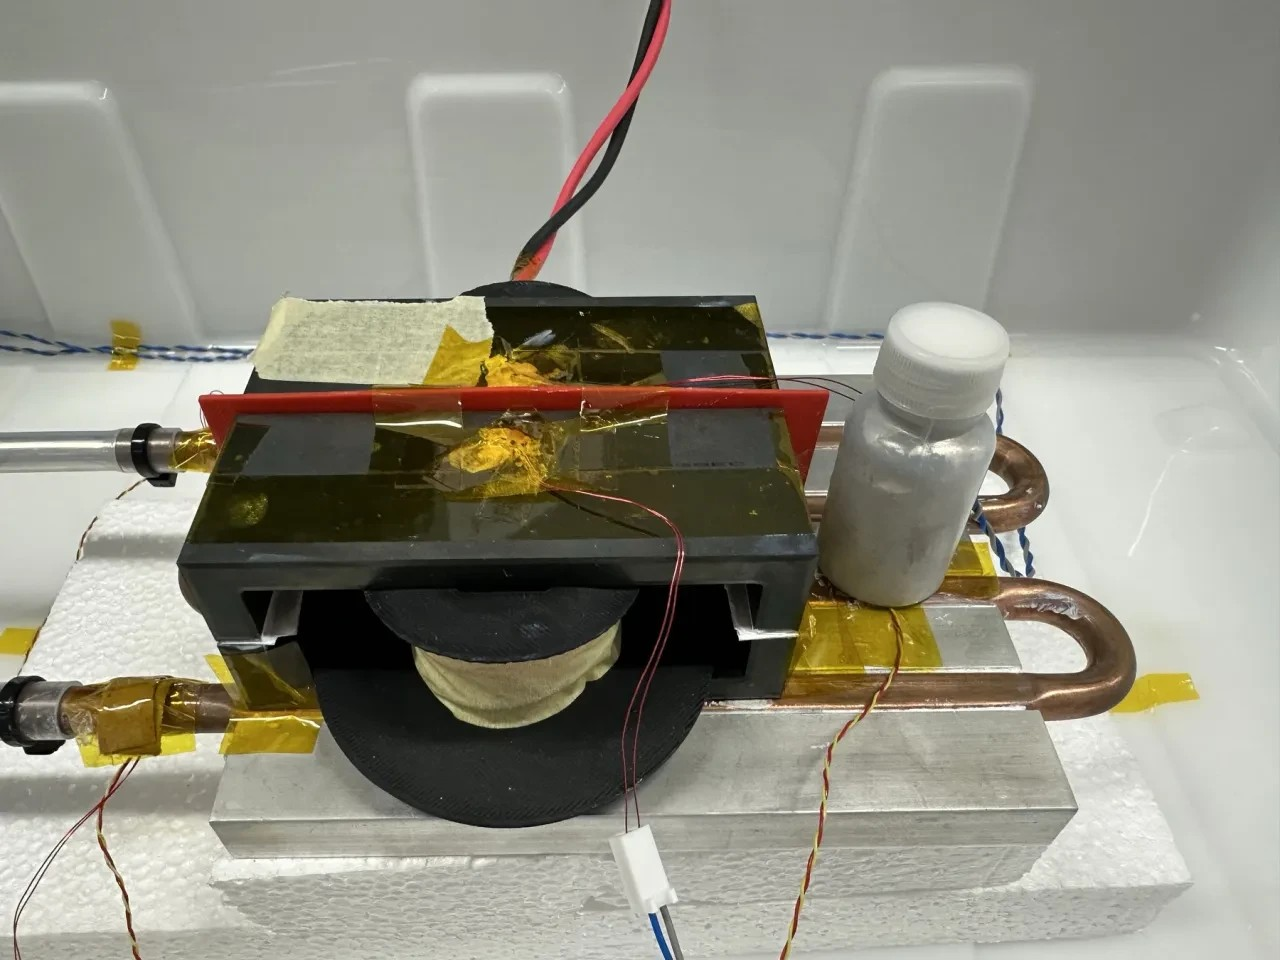
\includegraphics[width=0.6\linewidth]{inductor_vial_setup}
  \caption{Inductor on the Galinstan cold plate, with the PVC vial of Galinstan
    standing beside it, as used for configuration~(iv) of the eddy-current loss
    measurement.}
  \label{fig:vial-setup}
\end{figure}
